%% \chapter[htoc-titlei][hhead-titlei]{htitlei}
%% -----------------------------------------------------------------------------
\chapter[Statistical interpretation technique][Statistical interpretation]
        {Statistical interpretation technique}
\label{apx:stat_interpretation}

\begin{quote}
  Statistical interpretation is a critical part of any Physics analysis.
  It is used in many aspects of an analysis, including background fits,
  and to translate the observation into a result, either a discovery
  or an exclusion.

  The analysis presented in this thesis uses a maximum likelihood fit to the
  data to obtain a background fit.
  The particular likelihood function uses for this analysis is described in
  Section~\ref{apx:likelihood}.
  Ultimately, the \cls\ method is used to set exclusion limits on the stop
  mass and branching fraction.
  The \cls\ method uses a modified frequentest technique, and is described
  in Section~\ref{apx:cls}.
\end{quote}

%% -----------------------------------------------------------------------------
\section{Likelihood function}
\label{apx:likelihood}

This analysis uses a maximum likelihood fit to determine the normalization
factors of the major backgrounds, and to constrain the systematic uncertainties
based on the observations in the signal and control regions.

The maximum likelihood treats the systematic uncertainties as ``nuisance
parameters,'' which are profiled using a Gaussian distribution.
This means the size of a particular uncertainty can be further
constrained (or made larger) compared to the nominal value based on the
compatibility of the data with the prediction.
The Gaussian distribution applies a penalty in the likelihood function for
varying the nuisance parameters to ensure the cannot float freely.

The most general form of the maximum likelihood function used in this analysis
incorporates several signal and control regions, referred to as ``channels,''
where each channel may have several bins.
A template form of the maximum likelihood function can be written as
\begin{equation}
  \mathcal{L}\left(
    \mathbf{n},
    \boldsymbol{\vartheta}
    \given
    \mu_\mathrm{sig},
    \boldsymbol{\mu}_\mathrm{bkg},
    \boldsymbol{\vartheta}
  \right) =
  % \prod_{c \in \mathrm{channels}}
  % \prod_{b \in \mathrm{bins}}
  \prod_{\substack{c \in \mathrm{channels} \\ b \in \mathrm{bins}}}
  \underbrace{
    % \mathrm{Pois}
    P
    \left( n_{cb} \given
      \nu_{cb} \left(
        \boldsymbol{\mu}_\mathrm{sig},
        \boldsymbol{\mu}_\mathrm{bkg},
        \boldsymbol{\theta}
      \right)
    \right)
  }_{\substack{\text{Poisson for each bin}\\\text{in each channel}}}
  \,
  \cdot
  \,
  \prod_{p \in \substack{\text{nuisance} \\ \text{parameters}}}
  \underbrace{
    % \mathrm{Gaus}
    G
    \left(\vartheta_{p} \given \theta_{p} \right)
  }_{\substack{\text{Gaussian}\\\text{constraints}}},
  \label{eqn:template_likelihood}
  \end{equation}
where the parameters can be interpreted as
\begin{description}
  \item[$\mathbf{n_{cb}}$:] 
    The number of \textbf{observed} events in channel $c$ and bin $b$.
  \item[$\boldsymbol{\nu_{cb}}$:] 
    The \textbf{expected} number of events in channel $c$ and bin $b$.
    These quantities depend on the other parameters that enter the likelihood.
  \item[$\boldsymbol{\vartheta_{p}}$:] 
    The \textbf{best fit} value for for the nuisance parameter $p$.
    These quantities are varied to achieve a maximum likelihood, but there is
    a penalty associated with these variations.
  \item[$\boldsymbol{\theta_{p}}$:] 
    The \textbf{nominal value} for for the nuisance parameter $p$.
  \item[$\boldsymbol{\mu_\mathrm{sig}}$:]
    Normalization factor of the signal sample.
    This quantity is allowed to vary without penalty.
  \item[$\boldsymbol{\mu_\mathrm{bkg}}$:]
    Vector of the normalization factors of the background samples.
    There is one normalization factor for each background process who's
    normalization is allowed to vary.
    The components of $\boldsymbol{\mu_\mathrm{bkg}}$ are allowed to vary
    independent of one another, and as with $\mu_\mathrm{sig}$, there is no
    penalty for these variations
\end{description}
The first term in Equation~\ref{eqn:template_likelihood} is a product of
Poisson functions, where the product is taken over each of the channels
($c$) considered and the bins ($b$) within each channel.
The analysis described in this thesis does not used binned signal and control
regions
The product is only be taken over the channels in this situation.
The second term is a product of Gaussian functions, taken over each of the
systematic uncertainties, taken as nuisance parameters.

In order to find the normalization factors~($\mu_\mathrm{sig}$ and
$\boldsymbol{\mu_\mathrm{bkg}}$) and nuisance
parameters~($\boldsymbol{\vartheta}$) which maximize the likelihood function, 
$-\log \mathcal{L}$ is minimized.
The log-likelihood function is easier to work with numerically because the
raw likelihood spans many orders of magnitude, so the gradient is very steep.
The negative of the log-likelihood is a convention often used, but not
meaningful.

%% -----------------------------------------------------------------------------
\section{The $CL_{s}$ method}
\label{apx:cls}

The search results presented in this thesis are interpreted using the \cls\
technique.
\cls\ is a method for determining limits developed at LEP, but is commonly used
in analyses on \atlas.
It is, at its core, a frequentest technique, but it does adopt some Bayesian
properties~\cite{0954-3899-28-10-313,2011EPJC...71.1554C}.

When making a discovery, a $p$-value test is commonly used to evaluate the
confidence level of the result.
The background-only model is declared the ``null hypothesis,'' and the 
``alternate hypothesis'' is defined as the scenario where the data contain both
signal and background events.
The observation is compared with the prediction from the background-only
hypothesis, and if the data is incompatible ($p$-value less than some
threshold, $\alpha$), the null hypothesis is rejected, and the alternate
hypothesis is accepted with a confidence level of $(1-\alpha)$.

\begin{figure}[t]
  \centering
  \subbottom[Large separation]{
    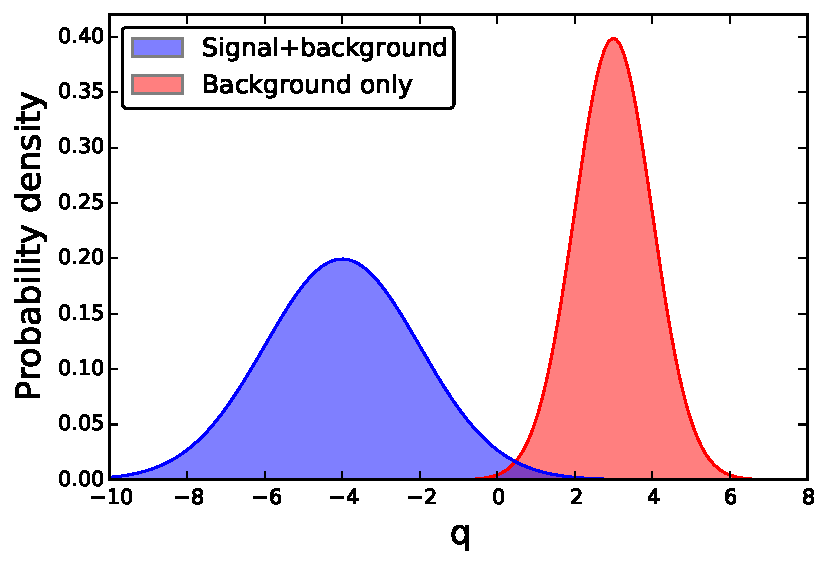
\includegraphics[width=0.45\textwidth]{figs/stats/pdf_large_separation.pdf}
    \label{fig:example_pdf_large_sep}
  }
  \subbottom[Small separation]{
    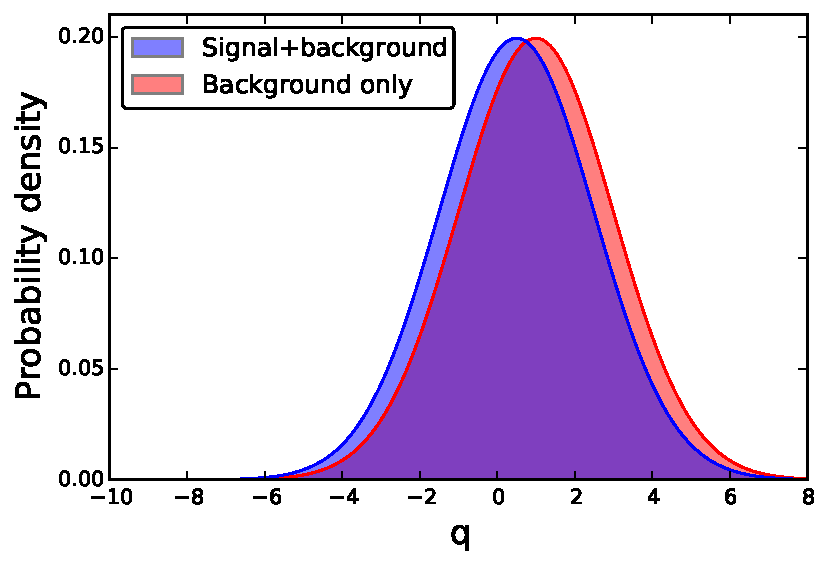
\includegraphics[width=0.45\textwidth]{figs/stats/pdf_small_separation.pdf}
    \label{fig:example_pdf_small_sep}
  }
  \caption{
    Examples probability distribution functions for signal+background and
    background-only hypotheses.
  }
  \label{fig:example_pdfs}
\end{figure}

While the $p$-value test is useful for evaluating a discovery, but if the
data is found to be compatible with the prediction, limits can be set, where
signal models are rejected if they are expected to be observed in the available
data.
One method that was commonly used in particle physics is the \clsb\ technique.
This technique defines a test statistic
\begin{equation}
  q\left( \mu \right) =
  -2 \ln
  \frac{\mathcal{L} \left( \mu, \boldsymbol{\theta} \right)}
  {\mathcal{L}_\mathrm{max}},
\end{equation}
where $\mathcal{L}$ is a likelihood ratio, $\mu$ is the signal strength being
tested, and $\boldsymbol{\theta}$ are the values of the nuisance parameters
which maximize the likelihood ratio.
The test statistic is calculated for the observation in the analysis regions, 
and the quantity \clsb\ is defined in such a way to give the probability
of a measurement at least as extreme as the observed test statistic.
If the observed test statistic is greater than the mean of the expected
signal+background probability distribution function, \clsb\ is defined as
\begin{equation}
  \clsb = \int_{q_\mathrm{obs}}^{\inf} P\left(q\left(\mu\right)\right) dq.
\end{equation}
\clsb\ is treated similar to a $p$-value for the signal+background model with
signal strength equal to $\mu$.
That is, if $\clsb < \alpha$ (where $\alpha$ is often set to 0.05), the signal
model with signal strength, $\mu$, is rejected with a $(1-\alpha)$ confidence
level.

The \clsb\ technique works well in scenarios where the test has good
statistical significance, as shown in Figure~\ref{fig:example_pdf_large_sep}.
If, however, the background-only and the signal+background hypotheses are not
well separated, as shown in Figure~\ref{fig:example_pdf_small_sep}, the
\clsb\ technique can (and does) reject signal models in favor of the
background-only hypothesis, when the data is incompatible with both!

The \cls\ technique provides protection from this sort of error by including
the agreement with the background-only hypothesis.
The compatibility of the observation with the background-only hypothesis is
\begin{equation}
  \clb = \int_{q_\mathrm{obs}}^{-\inf} P\left(q\left(\mu=0\right)\right) dq,
\end{equation}
assuming $q_\mathrm{obs}$ less than the mean of the expected background-only
probability distribution function.

\begin{figure}[t]
  \centering
  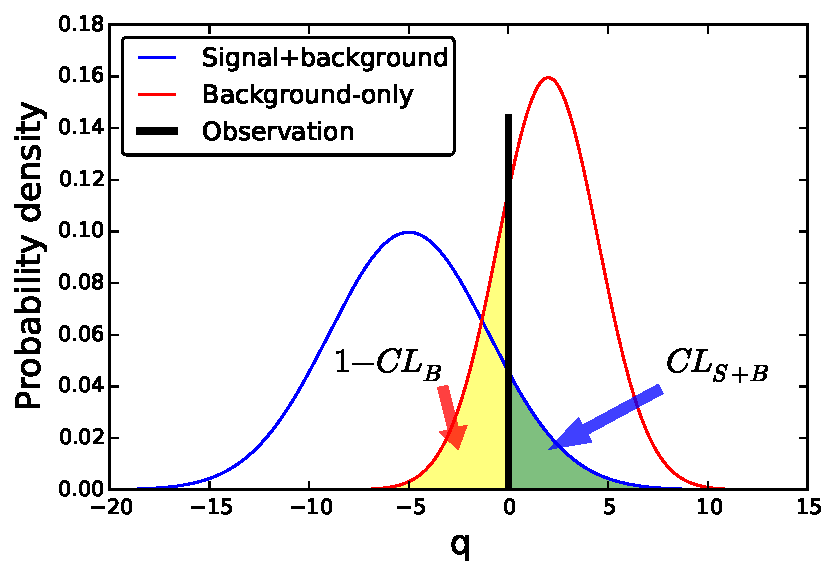
\includegraphics[width=0.80\textwidth]{figs/stats/cls.pdf}
  \caption[
    Examples probability distribution functions used to calculate the
    \cls\ quantity.
  ]{
    Examples probability distribution functions used to calculate the
    \cls\ quantity.
    The area shaded in red and blue are equal to \clb\ and \clsb\ respectively,
    and \cls\ is given by taking the ratio of the two.
  }
  \label{fig:cls}
\end{figure}

The \clsb\ and \clb\ quantities are used to construct \cls, which is defined as
\begin{equation}
  \cls = \frac{\clsb}{\clb},
\end{equation}
An example of the application of the \cls\ method is shown in
Figure~\ref{fig:cls}.
The two curves represent the expected probability distributions for the
signal+background hypothesis (blue) and the background-only hypotheses (red),
and the black line is placed at the value of $q$ corresponding to the
observation.
The shaded areas are equal to the \clsb\ (green) and $1-\clb$ (yellow), thus
\cls\ is equal to the ratio of these areas.

The \cls\ value is penalized if the data is incompatible with both the
signal+background and background-only hypotheses or if the two hypotheses are
indistinguishable.
This is particularly important when the number of expected and observed events
is low, leading to large statistical uncertainties.
In these cases, a downward fluctuation of only a few events may result in a
signal model being excluded by the \clsb, but the \cls\ method tends to be
more conservative in this respect.
